%% The first command in your LaTeX source must be the \documentclass command.
%%
%% Options:
%% twocolumn : Two column layout.
%% hf: enable header and footer.
\documentclass[
% twocolumn,
% hf,
]{ceurart}

%%
%% One can fix some overfulls
\sloppy

%%
%% Minted listings support
%% Need pygment <http://pygments.org/> <http://pypi.python.org/pypi/Pygments>
\usepackage{listings}
%% auto break lines
\lstset{basicstyle=\ttfamily,breaklines=true}

%%% Colors
\definecolor{light-gray}{RGB}{245,245,245}
\definecolor{darkgreen}{RGB}{0, 153, 0}
\definecolor{iri}{RGB}{0,0,0}
\definecolor{prefix}{RGB}{0,0,195} %dark blue
\definecolor{afterPrefix}{RGB}{0,0,245}
\definecolor{colorcomment}{RGB}{0, 153, 0}
\definecolor{mahogany}{RGB}{153,0,0}
\definecolor{darkblue}{RGB}{0,0,200}


%%%Turtle
\lstdefinelanguage{turtle}
{
  identifierstyle=\color{afterPrefix},    %afterPrefix
  morecomment=[n][\color{iri}]{<}{>}, % iris
  morestring=[b][\color{black}]{\"},  % strings
  % -------------------------- prefixes
  classoffset=1,
  keywordstyle=\color{prefix},
  morekeywords={dcterms, owl, rdfs, rdf, schema, reg, skos, xsd, sh},
  % -------------------------- rdfType
  classoffset=2,
  keywordstyle=\color{purple},
  morekeywords={a},
  % -------------------------- language
  classoffset=3,
  keywordstyle=\color{orange},
  morekeywords={@en}
}

%%% SPARQL
\lstdefinelanguage{SPARQL}
{
  morecomment=[l][\color{gray}]{\#},       % comments
  morecomment=[n][\color{black}]{<http}{>}, % uris
  morestring=[b][\color{black}]{\"},  % strings
  % -------------------------- variables
  keywordsprefix=?,
  classoffset=0,
  keywordstyle=\color{darkblue},
  morekeywords={},
  % -------------------------- prefixes
  classoffset=1,
  keywordstyle=\color{orange},
  morekeywords={act,dcterms,ncit,rdf,schema},
  % -------------------------- keywords
  classoffset=2,
  keywordstyle=\color{purple},
  morekeywords={ASK,a,PREFIX}
}

%%%Enironment for diagram
\usepackage{tikz}
\usetikzlibrary{positioning}
\usetikzlibrary{arrows.meta}
\tikzset{%
  >={Latex[width=2mm,length=2mm]},
  % Specifications for style of nodes:
    base/.style = {rectangle, rounded corners, draw=black,
                   minimum width=2.5cm, minimum height=1cm,
                   text centered, font=\sffamily\small, fill=white},
  result/.style = {base, fill=orange}
}

%%
%% end of the preamble, start of the body of the document source.
\begin{document}
%%%URLs in footnotes, that have #
\urldef\urlshacltargets\url{https://www.w3.org/TR/shacl/#targets}
\urldef\urlshaclprebinding\url{https://www.w3.org/TR/shacl/#pre-binding}
\urldef\urlschaclgraphdata\url{https://www.w3.org/TR/shacl/#data-graph}
\urldef\urlshaclconstraintcomponent\url{https://www.w3.org/TR/shacl/#sparql-constraint-components}

%%
%% Rights management information.
%% CC-BY is default license.
\copyrightyear{2023}
\copyrightclause{Copyright for this paper by its authors.
Use permitted under Creative Commons License Attribution 4.0
International (CC BY 4.0).}
\conference{KGCW'23: 4th International Workshop on Knowledge Graph Construction, May
28, 2023, Crete, GRE}

%%
%% The "title" command
\title{Test-driven Knowledge Graph Construction}


%%
%% The "author" command and its associated commands are used to define
%% the authors and their affiliations.
\author[1]{Jindřich Mynarz}[%
email=mynarzjindrich@gmail.com,
]
%\cormark[1]
%\fnmark[1]
\address[1]{Department of Information and Knowledge Engineering, Prague University of Economics and Business \\ Nám. W. Churchilla 4, 130 67, Praha 3, Czech Republic}

\author[1]{Kateřina Haniková}[%
email=hank05@vse.cz,
]

\author[1]{Vojtěch Svátek}[%
email=svatek@vse.cz,
]

%%
%% The abstract is a short summary of the work to be presented in the
%% article.
\begin{abstract}
  We propose how to construct knowledge graphs using a method based on user requirements formulated as competency questions. It suggests to formalize the competency questions as SPARQL queries wrapped as SHACL constraints allowing them to be used as automated tests. The method defines a process to guide knowledge graph construction by feedback from tests. It aims to reduce the engineering effort required to construct a knowledge graph that meets the requirements, while assessing the quality of semantic artifacts produced in this effort. We intend the method to provide a solid engineering basis for knowledge graph construction that uses the lessons learnt from software development and is built on open standards. We demonstrate using the method to construct a knowledge graph about antigen covid tests and reflect on the proposed method.
\end{abstract}

%%
%% Keywords. The author(s) should pick words that accurately describe
%% the work being presented. Separate the keywords with commas.
\begin{keywords}
  testing \sep
  test-driven approach \sep
  knowledge graphs \sep
  competency questions
\end{keywords}

%%
%% This command processes the author and affiliation and title
%% information and builds the first part of the formatted document.
\maketitle

\section{Introduction}
Knowledge graphs use graph-based data models to capture knowledge commonly combined from large and diverse data sources \cite{Hogan2021}. Constructing knowledge graphs can be an intricate and open-ended task that is in many ways an art rather than a craft.\footnote{The same argument was made about designing ontologies by Soldatova et al. \cite{Soldatova2016}.} While there are resources covering \textit{how} to build knowledge graphs, there is little on \textit{what} to build: how to elicit, formulate, and validate requirements for a knowledge graph. Overall, there is a shortage of solid engineering practices guiding through this task.

We propose how to construct knowledge graphs using a standards-based method founded upon user requirements formulated as competency questions (CQs). It suggests to formalize the CQs as SPARQL queries \cite{SPARQL2013} and wrap them as SHACL constraints \cite{SHACL2017} in order to allow them to be executed as automated tests. The method defines a process guiding knowledge graph construction that is based on feedback from tests. It aims to reduce the effort required to construct a knowledge graph that meets its requirements and passes quality assessment of semantic artifacts, such as ontologies, that are made in the process.

\section{Motivation}
Following a method for knowledge graph construction offers several benefits. In general, a~method helps decide what to do next. In particular, it helps to overcome the blank canvas paralysis at the beginning and jump-start the work. Moreover, a method breaks down the effort required for knowledge graph construction into sub-tasks, which can help organize and coordinate a team working on them.

The direction provided by a method anchored in user requirements can reduce the unfocused upfront effort and help avoid over-engineering. For example, it discourages needless effort spent on achieving a lossless transformation that preserves all source data in the produced knowledge graph even though it might not be needed. It can help avoid premature abstraction and premature optimization, such as for performance or readability. Thanks to the tests checking if the user requirements are satisfied, we get an early proof of value instead of speculating about it. Additionally, the explicit links between requirements and tests allow to assess the requirements traceability and coverage.

\section{Related Work}
When outlining this method, we can learn from ontology engineering, as it has a head start of several decades on knowledge graphs. There is a long tradition of using competency questions as requirements for ontologies \cite{Gruninger1994}. Much of this experience can be reused, since ontologies serve as essential building blocks of knowledge graphs imbuing them with explicit semantics. Knowledge graphs in turn can be considered as ontologies populated with data. Creating tests for ontologies out of CQs is also nothing new \cite{Ren2014,Zemmouchi2013}. More recently, it was adopted for knowledge graphs too \cite{Pan2017}.

Broader still, we can adopt the practices established in software engineering. The hereby presented method borrows from the test-driven development cycle \cite{Beck2003}, which is commonly characterized by the following steps:
\begin{itemize}
    \item Add a test
    \item Run all tests, expecting the new test to fail
    \item Write the simplest code that passes the new test
    \item All tests should pass
    \item Refactor as needed
\end{itemize}

A fundamental feature of this cycle is that it intertwines development with testing, so that tests exercise the developed artifacts and provide feedback informing further work. Tests provide a controlled way to evolve the artifacts under construction in response to changing requirements, such as when their scope is extended or when they are refined iteratively. The field of ontology engineering is already adopting agile development approaches using tests. Ontology-specific methods, such as SAMOD \cite{Peroni2016} or Linked Open Terms \cite{PovedaVillalon2022}, are being proposed.

In summary, the hereby described method borrows approaches either from ontology engineering or software development in general and proposes a novel way how to combine them for knowledge graph construction. The following text characterizes the method and demonstrates its use for building a knowledge graph about antigen covid tests.

\section{Method}
\begin{figure}
\centering
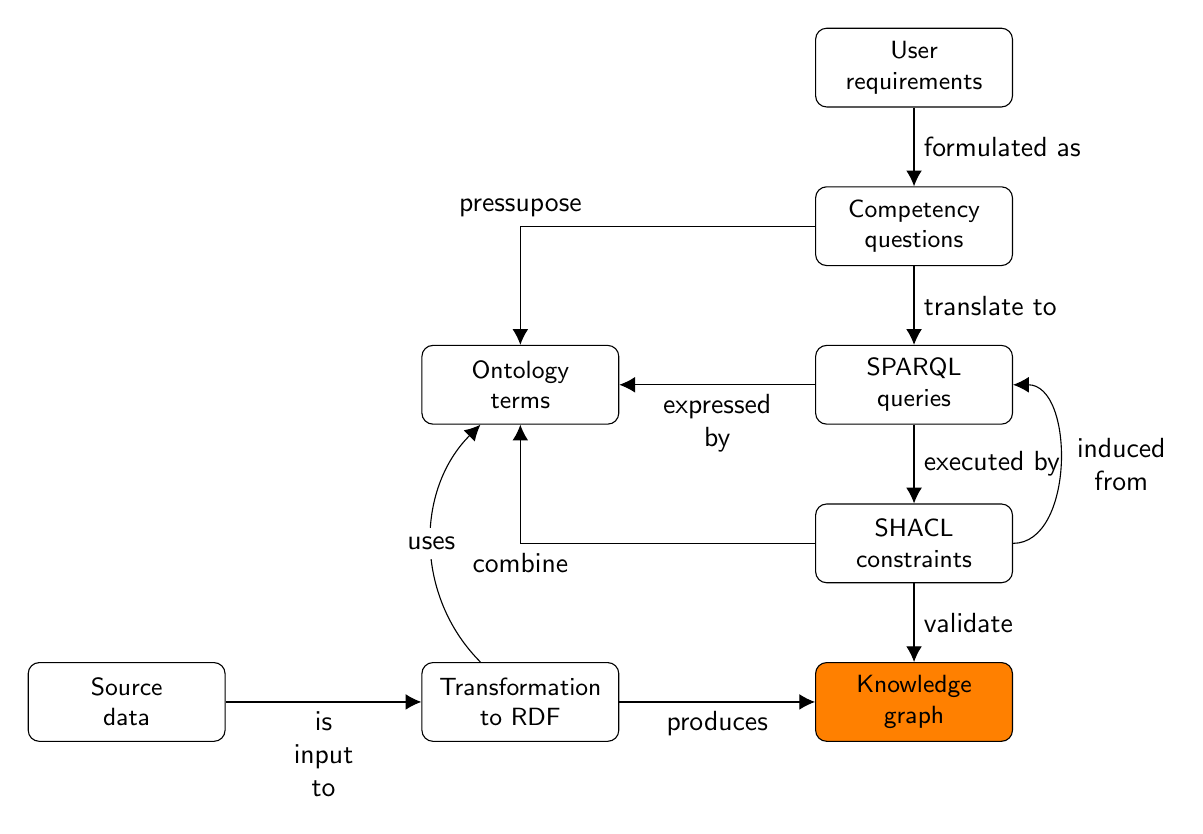
\begin{tikzpicture}[node distance=1.5cm, every node/.style={fill=white, font=\sffamily}, align=center, tips=proper]
  \node (requirements)   [base]                                             {User\\requirements};
  \node (cqs)            [base, below=1cm of requirements]                      {Competency\\questions};
  \node (sparql)         [base, below=1cm of cqs]                               {SPARQL\\queries};
  \node (shacl)          [base, below=1cm of sparql]                            {SHACL\\constraints};
  \node (kg)             [result, below=1cm of shacl]                           {Knowledge\\graph};
  \node (ontology)       [base, left of=sparql, xshift=-3.5cm]                             {Ontology\\terms};
  \node (transformation) [base, left of=kg, xshift=-3.5cm] {Transformation\\to RDF};
  \node (source)         [base, left of=transformation, xshift=-3.5cm]        {Source\\data};

  % Specification of lines between nodes specified above
  % with aditional nodes for description
  \draw[->]      (requirements) -- node[right] {formulated as} (cqs);
  \draw[->]               (cqs) -- node[right] {translate to} (sparql);
  \draw[->]               (cqs) -| node[above] {pressupose} (ontology);
  \draw[->]            (sparql) -- node[right] {executed by} (shacl);
  \draw[->]            (sparql) -- node[below] {expressed\\by} (ontology);
  \draw[->]             (shacl) -- node[right] {validate} (kg);
  \draw[->]             (shacl.east) edge[bend right=90] node[right, xshift=0.1cm] {induced\\from} (sparql.east);
  \draw[->]            (source) -- node[below] {is\\input\\to} (transformation);
  \draw[->]    (transformation) -- node[below] {produces} (kg);
  \draw [->] (transformation) edge[bend left=45] node {uses} (ontology);
  \draw[->]             (shacl) -| node[below] {combine} (ontology);
\end{tikzpicture}
\caption{Knowledge graph construction method} \label{fig:process}
\end{figure}


We present a method for test-driven knowledge graph construction. The method proposes a~sequence of steps and feedback loops between them. Each step produces or consumes one or more artifacts, such as ontologies or SPARQL queries. An overview of the relations between the key artifacts used by the method is depicted in Figure \ref{fig:process}. The method involves the following steps:
\begin{enumerate}
    \item Start by using knowledge elicitation techniques \cite{Shadbolt2015} to gather user requirements. User requirements can be gathered from subject-matter experts or prospective users of the knowledge graph. Formulate the user requirements as CQs \cite{Gruninger1994}. CQs are analytical questions that the target knowledge graph is expected to answer. In order to avoid misinterpretation, they should be reviewed by those who expressed the requirements the~CQs capture.
    \item Analyze the CQs to extract terms and relations. CQs can be analyzed using the linguistic notion of presupposition, which can be defined as \textit{"a condition that must be met for a~linguistic expression to have a denotation"} \cite{Ren2014}. Viewed this way, CQs presuppose the terms with which they can be expressed. The terms to extract from CQs are typically nouns or noun phrases that refer to entities from the domain of the knowledge graph under construction. They can be considered lexical surface forms of these entities. The~terms can be identified manually or with the help of tools, such as part-of-speech tagging. The~relations to extract might be represented by verbs connecting the terms co-occurring in a CQ. Less direct mappings between entities and surface forms are possible too, such as when a surface form provides the context disambiguating an entity.
    \item Formalize the terms and relations in a minimum viable ontology using RDF Schema \cite{Brickley2014}. While terms typically map to classes (i.e. instances of \texttt{rdfs:Class}), relations map either to properties (i.e. instances of \texttt{rdf:Property}) or n-ary relations represented by classes. Document the ontology with definitions sourced from and validated by subject-matter experts to create a shared understanding. The ontology should make minimal ontological commitment to aid its evolution, so limit its upfront axiomatization, such as by using OWL restrictions. The resulting ontology shall serve as an explicit and machine-readable conceptualization of the knowledge graph's domain. Formalizing the ontology may in turn reveal ambiguity in the CQs. Ambiguous CQs cannot be formalized reliably since their misinterpretations may occur. In such cases, the sources of ambiguity should be revised with subject-matter experts while aiming to reformulate the CQs in an unambiguous way.
    \item Translate the CQs to SPARQL queries expressed by the ontology. SPARQL queries make the CQs executable. Here, we expect a manual translation of the CQs to SPARQL queries. Automated translation was attempted by others, such as in \cite{EspinozaArias2022}. Start with syntactically valid SPARQL queries of hypothetical data expressed by the ontology. A CQ may translate to a SPARQL graph pattern composed of triple patterns joining the terms co-occurring in the question via specific relations. The way CQs should be translated to SPARQL queries largely depends on their expected answers. Ren et al. \cite{Ren2014} suggest that we might be \textit{"more interested in checking if a CQ can be meaningfully answered, instead of directly answering a~CQ."} When using such existential quantification of the desired answers, a SPARQL query formalizing a CQ can be expected to return non-empty results. What it means is that the query can answer a~CQ using a~given knowledge graph. It does not verify if the answer is correct. Conversely, some CQs may describe universal invariants of their domain. Queries encoding these invariants are akin to property-based testing \cite{Fink1997}. In case stricter guarantees are needed, the expected correct answers can be included in the queries and validation constraints in SHACL implementing the CQs, corresponding to the usual example-based testing.
    \item Wrap the queries as SPARQL-based SHACL constraints to automate their execution. SHACL defines a target\footnote{\urlshacltargets} of each constraint. In our context, a target sets the scope of a CQ. The scope of the data graph validated by a given constraint may either encompass the entire knowledge graph or cover its subset. For instance, existentially quantified queries checking the complete data graph can target it by using \texttt{sh:targetNode []}. It is also possible to rewrite a part of a SPARQL query translating a CQ as target selection in SHACL. Alternatively, the prerequisite part of the query can be represented as a SPARQL-based target \cite{SHACLAF2017}. An~entity-centric partitioning of a given knowledge graph can be implemented by extracting concise bounded descriptions~\cite{Stickler2005} of the targeted entities. Some data sources of knowledge graphs may natively partition data to independent subsets, such as API responses or messages from a queue, that can be effectively validated by specific subsets of SHACL constraints. SHACL can also define the passing criteria of SPARQL-based constraints. An \texttt{sh:ask} query is expected to return the boolean \texttt{true}, while any results produced by an \texttt{sh:select} query are treated as violations. Specific expected results can be either hard-coded into the queries or specified via \texttt{sh:hasValue} in case a single value is expected. Note however, that when including the expected results in SPARQL-based constraints, we may run into the limitations of SHACL due to pre-binding of variables.\footnote{\urlshaclprebinding} For example, the \texttt{VALUES} clause, which could represent the expected results of \texttt{SELECT} queries, is not allowed.
    \item Develop a transformation of the source data to the target knowledge graph that is expected to meet the constraints. This can be implemented in many ways, largely dependent on the format of the source data, so we will not cover it here. For an overview of these approaches, see e.g., Fensel et al. \cite{Fensel2020b}
    \item Validate the knowledge graph under development with the SHACL constraints. If the validation fails, resolve the reported violations by fixing the artifacts created in the previous steps. Fix the most primary artifact causing the violations, i.e. their root cause. For instance, data transformation shall not work around an insufficiently expressive ontology. Similarly, imposing a more expressive data model on the knowledge graph might reveal errors in its source data. In this way, the finer structure of its ontology makes the previously hidden data quality issues visible. Some feedback may even indicate ill-formed CQs in need of revision.
    \item Refactor the artifacts. The SHACL specification of the knowledge graph is a key artifact to refactor. It can serve as a formal specification of the anticipated use of the ontology. Moreover, SHACL can transcend a single ontology and specify how to combine terms reused from multiple ontologies. During the refactoring, SHACL core constraints can be induced from SPARQL-based constraints to represent the frequently queried patterns in data. For instance, aided by the knowledge about the domain, you can infer universally quantified axioms represented as SHACL constraints from a sample of existentially quantified axioms represented as SPARQL queries. In particular, SHACL can prescribe the expected relations in data. More complex or distant relations might even require the expressivity of SHACL to be represented, using property paths or SPARQL graph patterns. For example, even though SHACL does not support conditional constraints directly, they can be rewritten according to the inference rule of material implication ${P\to Q\Leftrightarrow \neg P\lor Q}$.
\end{enumerate}

\section{Non-functional Requirements}

Note that the above-described method tests if a knowledge graph meets the given user requirements. It does not evaluate how well these requirements are satisfied. Absence of errors does not imply that the knowledge graph is sound. Therefore, the functional user requirements should be complemented by non-functional requirements describing the desired qualities of the solution. These requirements can be checked and refactored by using alternative sources of feedback, such as:

\begin{description}
    \item[Code review] \hfill \\
    Elicit expert insight from ontology and data engineers.
    \item[User feedback] \hfill \\
    The results produced by SPARQL queries formalizing the CQs can be judged to be incorrect by users. User feedback can identify wrong interpretation of CQs or false assumptions. It might prompt revisiting any of the previously described steps or lead to adding more CQs.
    \item[Usability testing] \hfill \\
    Usability may manifest in developer experience of writing SPARQL queries on a knowledge graph. In particular, complexity and verbosity of SPARQL queries may be considered. In this way, usability of the queries indirectly reflects the usability of the ontology. For example, verbosity may be caused by duplicate data that can be abstracted to the ontology, while complexity can be reduced by introducing ontological shortcuts. Verbose SPARQL queries may also suggest a need for introducing abstraction or additional axioms into the ontology. In fact, some CQs can be answered directly using the knowledge formalized in the ontology, since SHACL expects the validated data graph\footnote{\urlschaclgraphdata} to include the ontologies it populates.
    \item[Performance testing] \hfill \\
    Performance can be evaluated indirectly using the execution time of SHACL validation. This time is proportional to the execution times of the SPARQL queries the constraints include.
\end{description}

The non-functional requirements can also be covered by tests, such as query performance tests. These tests can provide additional feedback informing the test-driven development. Using the above-mentioned feedback is a balancing act of multi-objective optimization. For example, performance feedback may be incompatible with the feedback about verbosity or CQs may pose mutually conflicting requirements. Addressing the feedback thus requires making informed trade-offs.

\section{Limitations}

We are aware of several limitations of the proposed method. Here we recount some of them and suggest how to remedy them. The method may cause the developed artifacts outlined in the Figure \ref{fig:process} to overfit the user requirements in scope, which would hinder the reuse of the artifacts. This shortcoming can be remedied by including more CQs or focusing on reusability and abstraction during refactoring. User requirements for the knowledge graph under construction can be more complex than what SPARQL can express. One way around it is formalizing the requirements in a more expressive programming language that extends SHACL, such as in \cite{SHACLJS2017}. Ultimately, in order to ameliorate the limitations of this method, it is best combined with other methods, such as those for ontology design (e.g., Kendall and McGuinness \cite{Kendall2019}).

\section{Case Study: Antigen Covid Tests Knowledge Graph}

We used the described method to create a knowledge graph about antigen tests for SARS-CoV-2.

Its source data was originally gathered to create an overview of different evaluations of selected rapid antigen tests available on the Czech market.
Data analyses were carried out \cite{Kliegr2022} in order to validate the assumption that the claims on test quality provided by the manufacturers differ significantly from what is verified by the laboratories of independent organizations.

The data was collected manually from several regulatory bodies, such as SÚKL\footnote{\url{https://www.sukl.cz/prehled-testu-k-diagnostice-onemocneni-covid-19}} and EU HSC\footnote{\url{https://health.ec.europa.eu/health-security-and-infectious-diseases/crisis-management/covid-19-diagnostic-tests_en}}, and was combined with performance evaluations of the tests, such as their sensitivity and specificity, that came from independent studies from various countries.
The data was collected into an XML file.
The final destination of the data was originally twofold.
One was the actual portal that provided a graphical visualization of various properties of the tests.\footnote{\url{https://covidtesty.vse.cz/english/test-evaluation-older-data/}}
The other was a dashboard allowing to perform analyses online.
While the XML data was already structured, it lacked any ontological grounding, and some of its features were tuned towards presentation aspects within the website.

We set to create a knowledge graph out of it to open it to a wider reuse and allow performing retrospective analyses of this data.
All artifacts we developed in this effort, such as CQs, are available as open source\footnote{\url{https://github.com/KIZI/antigen-covid-tests-knowledge-graph}} and the knowledge graph is released.\footnote{\url{https://github.com/KIZI/antigen-covid-tests-knowledge-graph/releases/tag/v1.0.0}}

Understanding the source data and its domain was a key prerequisite of our work. The data covers 158 antigen SARS-CoV-2 tests and their evaluations from several sources. Each source had its way of describing the domain, which we needed to comprehend first to represent the source's data faithfully and make it commensurable. We also needed to become aware of the purpose for which the data was collected and how it was represented to serve this purpose. The data was originally structured in XML for display on a web page, so we needed to map its document-oriented structure and visual encoding into semantics. Knowing the source data well, we could begin with the knowledge graph construction.

\textbf{Step 1:} The first step of the proposed method is gathering user requirements. We started with capturing user requirements formulated as CQs, such as \textit{"What is the sensitivity of given tests according to their manufacturers?"} We came up with 19 CQs in total, covering both basic information look-up and more complex analytical questions. We removed one of the CQs later upon finding that it was subsumed by another CQ. The complete list of the CQs is available online.\footnote{\url{https://github.com/KIZI/antigen-covid-tests-knowledge-graph/wiki/Competency-questions}}

\textbf{Step 2:} We continued with analysis of the CQs and extraction of terms and relations, such as \textit{"sensitivity"}, \textit{"test"}, or \textit{"has manufacturer"} from the given example question. Since we did not have many CQs, we extracted the terms and relations manually.

\textbf{Step 3:} The third step was to create a minimum viable ontology from the extracted terms and relations, which we did mostly by reusing existing ontology terms and using RDF Schema; see Listing \ref{lst:example-onto}. For what we did not find suitable terms to reuse, we formalised terms in the simple Antigen Covid Test Ontology. This ontology aimed to allow expressing the CQs in SPARQL.

\begin{lstlisting}[language=turtle, caption=Example ontology terms, label={lst:example-onto}]
:DiagnosticSensitivity a rdfs:Class ;
  rdfs:label "Diagnostic sensitivity"@en .

:AntigenCovidTest a rdfs:Class ;
  rdfs:label "Antigen covid test"@en .

:hasManufacturer a rdf:Property ;
  rdfs:label "Has manufacturer"@en .
\end{lstlisting}

\textbf{Step 4:} Having a minimum viable ontology, we were able to translate the CQs into SPARQL queries, such as in the example Listing \ref{lst:example-cq-sparql}. Each question was translated manually.

\begin{lstlisting}[language=SPARQL, caption=Example competency question in SPARQL, label={lst:example-cq-sparql}]
PREFIX act:     <https://covidtesty.vse.cz/vocabulary#>
PREFIX dcterms: <http://purl.org/dc/terms/>
PREFIX ncit:    <http://purl.obolibrary.org/obo/NCIT_>
PREFIX rdf:     <http://www.w3.org/1999/02/22-rdf-syntax-ns#>
PREFIX schema:  <http://schema.org/>

ASK {
  ?test a act:AntigenCovidTest ;
    schema:manufacturer ?manufacturer .

  [] a ncit:C41394 ; # Diagnostic sensitivity
    dcterms:subject ?test ;
    dcterms:creator ?manufacturer ;
    rdf:value ?sensitivity .
}
\end{lstlisting}

\textbf{Step 5:} We wrapped the SPARQL queries as SHACL constraints, such as in the example Listing \ref{lst:example-cq} that defines a SPARQL-based constraint component\footnote{\urlshaclconstraintcomponent} applied to the entire data graph. The \texttt{sh:message} captures the CQ in natural language, which helps to identify which question failed to validate in the validation reports. The \texttt{sh:ask} contains the CQ translated to a SPARQL query prepared in the previous step.

\begin{lstlisting}[language=turtle, caption=Example competency question in SHACL,label={lst:example-cq}]
:DatasetShape a sh:NodeShape ;
  rdfs:label "Competency questions applicable to the entire dataset"@en ;
  sh:targetNode [] ;
  :cq12 [] .

:CQ12 a sh:ConstraintComponent ;
  rdfs:label "Manufacturer-declared test sensitivity"@en ;
  sh:parameter [
    sh:path :cq12
  ] ;
  sh:nodeValidator [
    a sh:SPARQLAskValidator ;
    sh:message """What is the sensitivity of given tests
                  according to their manufacturers?"""@en ;
    sh:prefixes :prefixes ;
    sh:ask """
    ASK {
      ?test a act:AntigenCovidTest ;
        schema:manufacturer ?manufacturer .

      [] a ncit:C41394 ; # Diagnostic sensitivity
        dcterms:subject ?test ;
        dcterms:creator ?manufacturer ;
        rdf:value ?sensitivity .
    }
    """
  ] .
\end{lstlisting}

\textbf{Step 6:} We started with implementing a transformation of the source data to RDF. We converted the input XML data into RDF/XML via an XSL transformation followed by SPARQL Update operations for post-processing. For example, we used post-processing for normalization of code-list values and manufacturers' names. We also implemented few traditional unit tests of XSL functions within the transformation.

\textbf{Step 7:} The resulting data was tested by the CQs implemented in SHACL. We automated the data processing and test execution by a shell script based on Jena command-line tools.\footnote{\url{https://jena.apache.org/documentation/tools}} Given that this is a small knowledge graph of around 10 thousand RDF triples, we validated it as a whole.

\textbf{Step 8:} The final step of the proposed method is about refactoring the developed artifacts. Our development work proceeded in several iterations guided by continuous feedback from the script for data transformation and validation. When the knowledge graph satisfied the CQs, we continued with refactoring the semantic artifacts we created. For example, we wanted to avoid blank nodes to make the data transformation results better comparable, so we improved the XSL transformation to generate IRIs instead. We also abstracted a parent class for evaluations in the ontology and adjusted the SHACL shapes accordingly.

Some errors were not detected by the tests implementing the CQs. For example, when querying the knowledge graph, we found that the data transformation to RDF mistakenly created IRIs of manufacturers based on their antigen covid test identifiers. Consequently, the resulting data related each manufacturer to one antigen covid test, so that it was not possible to group multiple tests by the same manufacturer. A common response to discovering errors not covered by tests is to improve the test coverage to enable detecting the errors found and avoid future regressions. We followed this practice and added a CQ comparing a given manufacturer's antigen covid tests. The CQ presupposed that there are manufacturers offering more than one test and would therefore fail in case of the above-described error. Apart from fixing the way we generated manufacturers' IRIs, we spent further effort on de-duplicating manufacturers via post-processing by SPARQL Update operations.

While we had CQs about manufacturers' tests, the implementations of these CQs generally asked if manufacturers' tests matching certain criteria exist. Being encoded as SPARQL ASK queries, any non-empty query results satisfied these CQs. They did not detect when the results were not the expected ones, such as when not showing all manufacturer's tests in the example of duplicate manufacturers above. We addressed this limitation by asking a more specific CQ presupposing more specific assertions. The more specific assertions we make about our domain, the better we can detect invalid data describing it. Yet when the domain changes or when our understanding of the domain is flawed, such assertions are more likely to become invalid. Consequently, there is a trade-off to be made between an assertion's specificity and its durability in face of change.

We encountered several other challenges during the development of the knowledge graph, such as handling the structure of the source data originally designed for a web presentation or frequent changes in relevant legislation and evaluation studies. Since the source data was collected manually, it was inconsistent and required fixes. Some of these inconsistencies manifested as duplicates and were detected by our test suite. Structuring the data as a knowledge graph and more rigorous testing thus helped to make the errors visible. Future work on this knowledge graph can be aimed at automatic updates of the data and expanding its coverage beyond the Czech market for antigen covid tests.

\section{Conclusions}

The hereby proposed method guides through the open-ended process of knowledge graph construction. It breaks the process down into a well-defined sequence of steps, feedback loops between them, and semantic artifacts that are produced or consumed in the process. The central contribution of the method is allowing to test if the produced knowledge graph satisfies the requirements for its construction. This is done via competency questions formulated as SPARQL queries embedded in SHACL shapes for test automation. As such, one of its key advantages is being based on the established semantic web standards.

We shared the experience of applying the method to build a knowledge graph about antigen covid tests. The method aided in collaborative development of this knowledge graph, allowing its incremental refinement without regressions. Since constructing knowledge graphs from the same user requirements using multiple methods, while comparing their outcomes, is prohibitively expensive, we expect future improvements of the proposed method to come from its applications on knowledge graphs with different requirements.

\begin{acknowledgments}
  This research was supported by CHIST-ERA within the CIMPLE project (CHIST-ERA-19-XAI-003).
\end{acknowledgments}
%%
%% Define the bibliography file to be used
\bibliography{resources}

\end{document}

%%
%% End of file
